\begin{savequote}[45mm]
\ascii{Any fool can write code that a computer can understand. Good programmers write code that humans can understand.}
\qauthor{\ascii{- Martin Flower}}
\end{savequote}

\chapter{OP本质论} 
\label{ch:essential-op}

\begin{content}

\end{content}

\section{OP的注册}

\begin{content}

在\cpp{}后端系统,系统初始化时,系统完成所有\ascii{OP}的注册。\ascii{OP}的注册是通过\code{REGISTER\_OP}宏完成的。

\subsection{REGISTER\_OP}

实施上,\code{REGISTER\_OP}定义了一套精致的内部\ascii{DSL},系统自动完成字符串表示的翻译表达,并将其转换为\code{OpDef}的内部表示,最后保存在\code{OpDef}的仓库中。

\begin{figure}[!h]
\centering
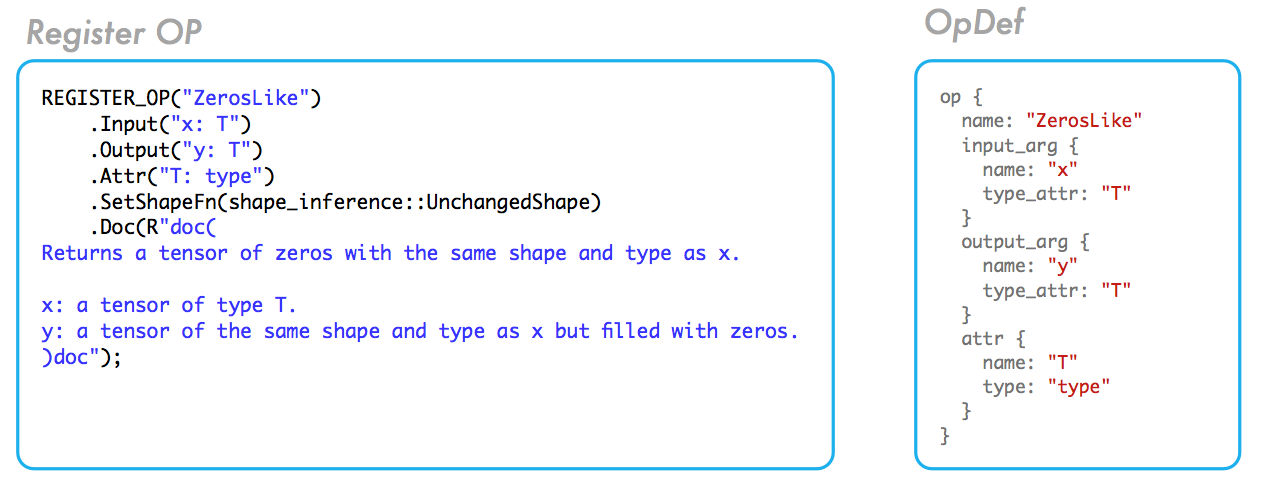
\includegraphics[width=0.9\textwidth]{figures/cc-op-repo.png}
\caption{REGISTER\_OP:注册OP的实用宏}
 \label{fig:cc-op-repo}
\end{figure}

\subsection{查询接口}

\begin{leftbar}
\begin{c++}
struct OpRegistryInterface {
  virtual ~OpRegistryInterface() {}

  virtual Status LookUp(
    const string& op_name,
    const OpRegistrationData** op_reg_data) const = 0;
  Status LookUpOpDef(const string& op_name, const OpDef** op_def) const;
};
\end{c++}
\end{leftbar}

其中,\code{OpRegistrationData}描述了\ascii{OP}两种基本的元数据:\code{OpDef}与\code{OpShapeInferenceFn};前者用于描述\ascii{OP}的输入/输出参数信息,属性名列表,及其约束关系。后者用于描述\ascii{OP}的\ascii{Shape}的推演规则。

\begin{leftbar}
\begin{c++}
struct OpRegistrationData {
  OpDef op_def;
  OpShapeInferenceFn shape_inference_fn;
};

using OpRegistrationDataFactory = 
  std::function<Status(OpRegistrationData*)>;
\end{c++}
\end{leftbar}

\subsection{OpDef仓库}

实现中,采用延迟初始化的技术。为了简化问题的描述,此处做了简单的代码重构,以便帮助大家理解\code{OpRegistry}的工作原理。

\begin{leftbar}
\begin{c++}
struct OpRegistry : OpRegistryInterface {  
  OpRegistry();
  ~OpRegistry() override;

  void Register(const OpRegistrationDataFactory& factory);

 private:
  Status LookUp(
     const string& op_name,
     const OpRegistrationData** op_reg_data) const override;

 private:
  using Registry = 
    std::unordered_map<string, OpRegistrationData*>;

  mutex mu_;
  Registry registry_;
};
\end{c++}
\end{leftbar}

\begin{leftbar}
\begin{c++}
Status OpRegistry::Register(
  const OpRegistrationDataFactory& factory) {
  auto op_reg_data(std::make_unique<OpRegistrationData>());
  Status s = factory(op_reg_data.get());
  if (s.ok()) {
    gtl::InsertIfNotPresent(&registry_, 
      op_reg_data->op_def.name(),
      op_reg_data.get())
  }
  Status watcher_status = s;
  if (watcher_) {
    watcher_status = watcher_(s, op_reg_data->op_def);
  }
  if (s.ok()) {
    op_reg_data.release();
  } else {
    op_reg_data.reset();
  }
  return watcher_status;
}
\end{c++}
\end{leftbar}

\end{content}